\chapter{Plataforma de desarrollo}
\label{cap:capitulo3}

\begin{flushright}
\begin{minipage}[]{6.5cm}
\emph{Lo simple es mejor que lo complejo.}\\
\end{minipage}\\

Tim Peters, \textit{The Zen of Python}\\
\end{flushright}

\vspace{1cm}
\setcounter{footnote}{1}

A continuación, se explican las plataformas de desarrollo utilizadas a nivel de software y hardware, que han permitido alcanzar los objetivos descritos en el capítulo anterior.

\section{Sistema operativo}
\label{sec:distribuicion}

Un sistema operativo puede definirse como el conjunto de programas que gestionan el hardware de un ordenador o dispositivo y permiten el funcionamiento de otros programas.
Como describen \cite{perales9a}, una distribución es una colección concreta de software de área de usuario y un núcleo del sistema operativo.

Para la realización de este proyecto se ha utilizado el sistema operativo de tipo GNU/Linux\footnote{\url{https://www.debian.org/releases/stable/i386/ch01s02.es.html}} y su distribuición Ubuntu\footnote{\url{https://ubuntu.com/}}, en concreto la versión Ubuntu 22.04.
La razón de usar esta versión de Ubuntu se debe a su compatibilidad con la distribuición \textit{Humble}\footnote{\url{https://docs.ros.org/en/humble/index.html}} de ROS 2, ya que el sistema ha sido diseñado específicamente para funcionar con dicha distribuición.

\section{Entorno de desarrollo}
\label{sec:entornos}

\subsection{Python}
\label{sec:entornos}

Python\footnote{\url{https://www.python.org/}} es el lenguaje de programación utilizado para el desarrollo de este proyecto.
Se trata de un lenguaje de alto nivel creado por Gido van Rossum y publicado por primera vez en 1991.
Según la documentación de \cite{perales9b} es un lenguaje ampliamente reconocido por su simplicidad y flexibilidad, lo que hace que sea ideal tanto para principiantes como para desarrolladores expertos. Cuenta con un sistema de tipos dinámico y gestión automática de la memoria y soporta múltiples paradigmas de programación, incluyendo orientación a objetos, programación funcional y estilos procedimentales. Además, dispone de una amplia y completa biblioteca estándar, que facilita el desarrollo de aplicaciones de propósito general.

La versión de Python utilizada para el desarrollo de la GUI es Python 3.10.13. En particular, se emplearon las siguientes librerías:

\begin{itemize}
    \item \textit{matplotlib:} Matplotlib\footnote{\url{https://matplotlib.org/}} es una biblioteca completa para crear visualizaciones estáticas, animadas e interactivas en Python. Se ha empleado para la graficación de las señales de trayectoria y perturbación, la posición del paciente en los entornos gamificados y de visualización del médico, y los datos clínicos recogidos durante la terapia.
    \item \textit{numpy:} NumPy\footnote{\url{https://numpy.org/}} es una biblioteca de Python que proporciona un objeto matriz multidimensional, varios objetos derivados como matrices y matrices enmascaradas y una serie de rutinas para realizar operaciones rápidas con matrices, incluidas operaciones matemáticas, lógicas, manipulación de formas, ordenación, selección, entrada/salida, transformadas discretas de Fourier, álgebra lineal básica, operaciones estadísticas simples, simulación aleatoria, entre otros. En especial se ha implementado dentro de los entornos gamificados para crear las señales límites, de trayectoría y perturbación para su posterior representación.
    \item \textit{tkinter:} Tkinter\footnote{\url{https://docs.python.org/es/3.13/library/tkinter.html}} es la interfaz por defecto de Python para el kit de herramientas de GUI Tk. En concreto, se han utilizado los módulos Tk y Ttk para el diseño de la interfaz de control del médico y la interfaz de registro de pacientes.
	\item \textit{pygame:} Pygame\footnote{\url{https://pypi.org/project/pygame/}} es una biblioteca multiplataforma gratuaita y de código abierto para el desarrollo de aplicaciones multimedia. Utilizada para incluir efectos de sonido dentro de un videojuego.
\end{itemize}\

\subsection{ROS 2}
\label{sec:entornos}

Como explica \cite{perales10a}, ROS\footnote{\url{https://www.ros.org/}} es un middleware que aumenta las capacidades del sistema para crear aplicaciones robóticas. El número dos indica que se trata de la segunda generación de este middleware.
Los paquetes de ROS 2 están organizados en distribuciones, las cuales están formadas por múltiples paquetes que aseguran su interoperabilidad.
Esta arquitectura modular permite estructurar el sistema como un grafo de computación, compuesto por nodos de ROS 2 que se comunican entre sí, permitiendo así que un robot realice una serie de tareas.

Se destacan las siguientes librerías:

\begin{itemize}
    \item \textit{rclpy:} rclpy\footnote{\url{https://docs.ros.org/en/iron/p/rclpy/}} proporciona la Interfaz de Programación de Aplicaciones (API) canónica de Python para interactuar con ROS 2.
    \item \textit{std\_msgs:} std\_msgs\footnote{\url{https://docs.ros2.org/foxy/api/std_msgs/index-msg.html}} define tipos de mensajes básicos y estandarizados para la publicación y suscripción entre nodos. Los tipos de mensajes utilizados en este proyecto son \verb|Int32|, \verb|Int32MultiArray|, \verb|Float32| y \verb|Float32MultiArray|.
\end{itemize}\

\section{Componentes físicos}
\label{sec:entornos}

Una vez definido el software, se especifica el hardware encargado de ejecutar las acciones en un entorno físico.
A pesar de que este trabajo se centra en el software del sistema, es importante conocer los dispositivos a utilizar y el propósito de los misos para desarrollar una arquitectura que se ajuste mejor a las necesidades y alcances del proyecto global.

Para el movimiento del brazo robótico se utiliza un actuador de HEBI Robotics\footnote{\url{https://www.hebirobotics.com/actuators}}, más concretamente el modelo T-Series como puede observarse en la Imagen \ref{fig:actuador}.
Este actuador está diseñado para funcionar como un componente robótico con todas las funciones.
La salida gira continuamente, no requiere calibración ni referencia alguna de arranque.
Diseñado para funcionar en brazos robóticos con múltiples grados de libertad.
Integra varios sensores facilmente accessibles a través de varias APIs.

La selección de este modelo se debe a la incorporación de un sensor de posición, lo que permite registrar el movimiento del brazo del paciente, así como su capacidad de control en fuerza al tratarse de un Sistema Electrónico de Actuación (SEA).
El sensor de posición resulta fundamental para la validación de los entornos gamificados, los cuales proponen una serie de actividades donde la posición del paciente se toma como referencia para el desarrollo de actividades interactivas y dinámicas dentro de un contexto terapéutico.
Además, el control por fuerza permite diseñar señales de tipo perturbación que simulan un nivel de resistencia o asistencia durante el ejercicio, lo que favorece la adaptación de la terapia a las capacidades de cada paciente.

\begin{figure}[ht!]
	\centering
	\begin{minipage}{0.45\linewidth}
		\centering
		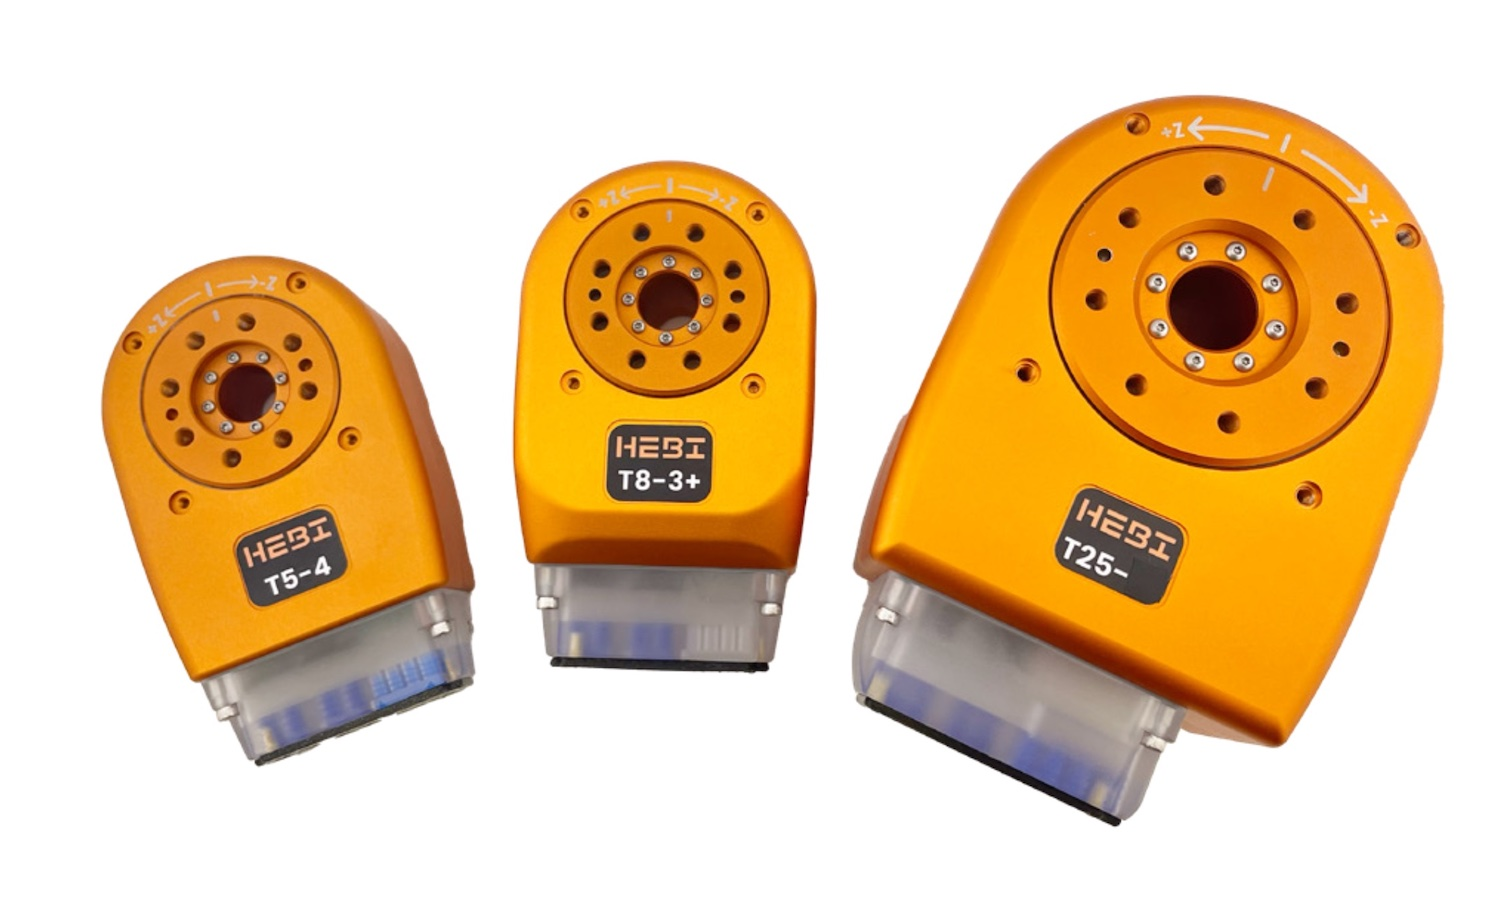
\includegraphics[width=\linewidth]{figs/actuador_T-Series.jpg}
	\end{minipage}
	\caption[Actuador T-Series]{Actuador T-Series}
	\label{fig:actuador}
\end{figure}
